\documentclass[9pt,twoside,lineno]{pnas-new}
% Use the lineno option to display guide line numbers if required.

%% Packages 
\usepackage{longtable}
\usepackage{csvsimple}



\templatetype{pnassupportinginfo}
% \readytosubmit %% Uncomment this line before submitting, so that the instruction page is removed.

\title{Association of Ebolavirus spillover events and annual birth pulses of African fruit bats}
\author{C. Reed Hranac, Jonathan C. Marshall, Ara Monadjem, David T. S. Hayman}
\correspondingauthor{David T. S. Hayman, E-mail: D.T.S.Hayman@massey.ac.nz}

\begin{document}

%% Comment/remove this line before generating final copy for submission
%\instructionspage  

\maketitle

%% Adds the main heading for the SI text. Comment out this line if you do not have any supporting information text.
\SItext


\section*{SI Methods}
\label{SI methods}

\subsection*{Chiropteran parturition data mining}
\label{dataMining}
African bat species that have been previous implicated in filovirus transmission either through RNA or antibody detection methods (see S1 Han et al. 2016 \cite{Han2016UndiscoveredFiloviruses,Walsh2005Wave-likeZaire}) were defined as the primary target for the data mining.
Targeted species were queried through Walker's Bats of the World \cite{Nowak1994WalkersWorld}, Scopus, Web of Science, and Google Scholar, using the generalized search terms: "Birth*"; "Breed*"; "Reproduc*"; "Partur*" along with the Latin binomial and common species names.
Bat species that had undergone taxonomic reassignment were queried under all names. Species that had been implicated, but did not reside in Africa, were queried on a genus level in attempt to identify representative sister species.
Preliminary results suggested insufficient sample sizes to model parturition on a per-species basis. Subsequently, the database was expanded to all mainland African bat and species were aggregated into three taxonomic clusters: Pteropodidae, Molossidae, and non-Molossid microbats, according to \cite{Cumming1997RainfallBats}, to account for the sharing of life history traits, including those associated with reproductive strategies and dietary preferences.
Publications returned from the queries were accessed by hand and when applicable, the location and month of parturition were extracted. Additional points for non-implicated species were added opportunistically as discovered and an African bat specialist (AM) was consulted to help fill holes in the dataset.
A total of 63 articles provided information on 14 pteropid species, 7 molossid species, and 43 non-molossid microbats at 75 number of unique locations totalling 165 event records (Figure 2 in the main text). Of these 88\% were retained and 8 locations were discarded as outside of our study extent.
Results are summarized in Supplemental Information Table ~\ref{table:DataMining}.\par

\subsection*{Covariate data}
\label{CoV}
	The spatial covariate data assembled to model and predict Chiropteran birthing and  EBOV spillover was blocked into two groups: static variables and temporally dynamic variables.
Our intention with this project is to capture the seasonality and phenology likely driving these events so the primary focus of our covariates were metrics capturing seasonality and change in the environment.
The static covariate layers were assumed to not vary between months of a year, be annually derived, or were not available for the different months of the year.
The static variables comprised: mammalian species biodiversity (computed from the IUCN distributions; see subsection below) \cite{IUCN2016TerrestrialData}; global land cover aggregated into `grassland', `forest', `urban' and `undefined' classes\cite{Olivier2012Global2009}; and four of the 19 Bioclimatic variables representing 30 year average for precipitation seasonality, mean diurnal range, temperature seasonality, and temperature annual range \cite{Frick2017WorldclimArease}.
Temporally dynamic covariates were all obtained at a monthly resolution and included layers describing mean monthly temperature, average monthly precipitation, potential evapo-transpiration \cite{Trabucco2009GlobalDatabase}; and an enhanced vegetative index \cite{Huete2002OverviewIndices}.
The study extent of the project was restricted to only the parts of Africa receiving more than 500mL of precipitation annually as suggested by \cite{Schmidt2017SpatiotemporalSpillover}.
All covariate layers were cropped and  masked to the precipitation layer, resolution was aggregated to ~25km raster blocks and temporally dynamic covariates were normalized (mean zero and standard deviation of 1). Extended Data Table ~\ref{table:ENM_CoV}

\subsubsection*{Mammalian diversity layers}
	layers were created to describe the number of species present at a location for a verity of criteria.
To create mammalian diversity raster layers the IUCN red list terrestrial mammals distribution database \cite{IUCN2016TerrestrialData} was used. Layers were created to describe total terrestrial mammalian diversity, non-Chiropteran terrestrial mammals, Pteropodidae, Molossidae, and non-Molossid microbats, as defined above using the \texttt{taxize} package \cite{Chamberlain2013Taxize:R} for taxonomic classification and manually checked by hand (see \texttt{DiversityRasters.R}).
The number of overlapping distributions for each cell within the study area were counted, and layers were cropped and masked to the study extent.
    
\subsubsection*{Land cover}
\label{Land cover}
The global land cover database \cite{Olivier2012Global2009} was obtained for the year 2009 and custom aggregation was used to reduce the number of classes from 23 to five as described but Supplemental Information Table~\ref{table:globReclass}.\par

\subsection*{Fragmentation index}
A binary mask of the aggregated `forest' class (as described above) from the Globcover 2009 dataset \cite{Olivier2012Global2009} was used to define forest patches using 4-connectivity.
A fragmentation index was then calculated for each pixel by counting the number of unique patches, within a 20x20 sliding window. \par

\subsection*{Human population}
Population density data were taken from the Worldpop (http://www.worldpop.org.uk) 2010 distribution for continental Africa.


 %   The occurrence/absence data and dimensionally reduced covariates were then modeled through the biomod2 ensemble modeling framework creating a single Chiropteran community-weighted ensemble model based on the receiver operating characteristic (ROC) score (see ~\ref{biomod}). Each Chiropteran community ensemble model was then re-projected across the study extent and transformed\todo[inline, color=orange]{What is the transformation here??} such that each cell represents $P(Birth_{y_x}$), the probability of birth occurring at location $x$ in month $y$. To account for Chiropteran diversity, the equation was used, where $\beta$ is the diversity of each taxonomic cluster at location $x$.\todo[inline, color=orange]{It's not clear to me how $\lambda$ is being used. I'm guessing this is in the model later on? Or is this for the bat birth surfaces. If so, I think you can drop the log? i.e. you just want a measure of 'bat births' so you have probability of bat birth times the diversity (which in this case is number of species I think?) which is kinda like the expected number of bat species giving birth?}


\subsection*{Biomod2 modeling}
\label{biomod}

To create continuous surfaces describing the presence or absence of bats giving birth for each of our taxonomic clusters we created a modified ecological niche modelling technique (ENM).
EMN require occurrence (or occurrence/absence) and co-variate data to create regressive correlations between observed environmental phenomena and observed distribution of events (generally speaking a species occurrence, in this case the birthing of young).
Data from the data mining was split by taxonomic grouping as described above and processed to create observation/absence data using a sliding two month window.
Records of a birth within the window were denoted as an occurrence and all locations for which data was present, but no births were recorded for the taxonomic group were deemed true absence points. 
The two month sliding window was chosen to reflect the non-discrete nature of birthing within wild animals as well accounting for data deficiencies.
An additional ten, randomly generated, down-weighted points (five occurrence and five absence points) were added to all models in order to insure the representation of all land cover categories in all models, and provide necessary pseudo-absence points in a small number of cases in which and insufficient number of absence points existed.
Covariate data was selected using Six month subsets of the temporally explicit covariates.
Selections were centred on the observation window and included the two preceding, and following months.
Due to the inherent correlation of the covariates (especially the temporally dynamic covariates) and general non-independence of all selected environmental covariates, a raster based PCA methods were used to reduce the dimensionality of all continuous predictors into six orthogonal principal components using the \texttt{rasterPCA} function of the package RSToobox.
The categorical land cover variable was then added to the other dimensionally reduced co-variates and occurrence/absence data were fed into the \texttt{biomod2} framework.\par

Procedurally generated ENMs were generated for all taxonomic clusters for all pairs of consecutive months where the number of combined observations was greater than 7.
Ten iterations of the potential eight preliminary models (generalized linear model, generalized boosted model, classification tree analysis, artificial neural network, surface range envelope, flexible discriminate analysis, random forest and maximum entropy) were computed using a standard 70:30 training:test ratio.
An ensemble model was then generated based on the weighted mean of the receiver operating characteristic (ROC score).
The resulting ensemble model was then projected back across the input data to produce a continuous probability surface of bat birthing for the study area. 
Model scores are summarized in Supplemental Information Table.\par

Ensemble mode results were combined with rasters describing the taxonomic beta diversity (as described above) to create a "Force of Birthing" metric $\lambda_{T,i,t}$ as described by:
 \begin{equation}
    \begin{gathered}
 	    \lambda_{T,i,t} = log(P(Birth_{T,i,t})*\beta_{T,i} +1)
    \end{gathered}
 \end{equation}
where for each taxonomic group $T$, at location $i$ and time $t$ number of taxonomic members is give by $\beta_{T,i}$, and the probability of birth occurrence is $P(Birth_{T,i,t})$.
relative number of members giving birth at any location in time and space. The abbreviations $ptr$, $mic$ and $mol$ were used to represent Pteropodidae, Non-Molossid Microbats, and Molossidae respectively.  

\subsection*{Modeling of outbreak events}
\label{spatGLM}
We fit a spatially weighted, overdispersed poisson general linear model (GLM) where log case rate is modelled as:
\begin{equation}
\begin{gathered}
\log(RR_{hum, l, i, t}) \sim \beta_1 \lambda_{ptr, l, i, t} + \beta_2 \lambda_{mic, l, i, t} + \beta_3 \lambda_{mol, i, t} \\
+ \beta_4 \lambda_{ptr, l-2, i, t} + \beta_5 \lambda_{mic, l-2, i, t} + \beta_6 \lambda_{mol, l-2 i, t} \\
+ \beta_7 \lambda_{ptr, l-4 i, t} + \beta_8 \lambda_{mic, l-4, i, t} + \beta_9 \lambda_{mol, l-4 i, t} \\
+ \beta_{10} \lambda_{ptr, l-6, i, t} + \beta_{11} \lambda_{mic, l-6, i, t} + \beta_{12} \lambda_{mol, l-6 i, t} \\
+ \beta_{13} RR_{an, l, i, t}* + \beta_{14} RR_{an, l-1, i, t}*  \\
+ \beta_{15} PopDen_{i}* + \beta_{16} NBM div_{i}* \\
+ \beta_{17} fragIndex_{i}* 
\end{gathered}
\end{equation}
where $RR_{hum}$ represents the relative risk of spillover events in humans, $\lambda_{T, l, i, t}$ is the force of birthing lagged by $l$ months.
The spillover into potential non-reservoir hosts at any pixel, time and lag is $RR_{an, l , i, t}$. Human population density, non-Chiropteran mammalian diversity, and a forest fragmentation were also included as the terms: $PopDen_{i}*$; $NBM div_{i}*$; and $fragIndex_{i}*$.
These three terms included no temporal aspects and were all transformed by $log +1$ denoted by $*$. \par 

	Spatial weights were used to account for spatial autocorrelation of cases and generated through the use of a \texttt{spatstat} quadrature scheme.
The quadrature was based on a raster grid of the same structure as those used throughout the the analysis. Relative risk values predicted back across sample space and reprojected.

\subsection{qAIC}
\label{qAIC}
Models with and without the force of birthing terms were compared using a quasi-Akaike information criteria (qAIC) scheme of the form: 
\begin{equation}
    \begin{gathered}
        qAIC = deviance X \hat{C} + 2k \\
        \hat{C} = \sum{weights * residuals^2}/df.residuals
    \end{gathered}
\end{equation}
Over dispersion was calculated by $\hat{C}$ and $k$ represents the number of terms.\\


%%% Each figure should be on its own page

%% Long table start
\setlength\tabcolsep{3.3pt}
\begin{longtable}{cccp{5cm}}
\caption{Caption for long table}\label{table:DataMining}\\
\multicolumn{1}{c}{\textit{Species}} & \multicolumn{1}{c}{Annual Births} & \multicolumn{1}{c}{Locations} & \multicolumn{1}{c}{References}\\
\hline 
\endfirsthead

\multicolumn{3}{c}%
{{\bfseries \tablename\ \thetable{} -- continued from previous page}} \\
\hline \multicolumn{1}{c}{\textit{Species}} & \multicolumn{1}{c}{Number Annual Births} & \multicolumn{1}{c}{Number Locations} & \multicolumn{1}{c}{References}\\ \hline 
\endhead

\hline \multicolumn{3}{|r|}{{Continued on next page}} \\ \hline
\endfoot

\hline \hline
\endlastfoot
\multicolumn{4}{l}{\textit{Pteropodidae}} \\
\hline \hline
\textit{Casinycteris ophiodon} & 1 & 1 & \cite{Wolton1982EcologicalMicrochiroptera} \\
\textit{Eidolon helvum} & 1-2 & 3 & \cite{Mutere1967The020N,Thomas1983ThePteropodidae,Funmilayo1979ECOLOGYNIGERIA,Fayenuwo1974BreedingNigeria}\\
\textit{Epomophorus gambianus} & 1-2 & 3 & \cite{COE1975MAMMALIANLIBERIA,Marshall1982EcologicalWoodland,Thomas1984ReproductionBats}\\
\textit{Epomophorus labiatus} & 2 & 1 & \cite{Okia1974TheUganda.}\\
\textit{Epomophorus wahlbergi} & 1-2 & 2 & \cite{Monadjem2012BreedingSwaziland,Wickler1976FieldCalling.}\\
\textit{Epomopos buettikoferi} & 2 & 2 & \cite{Thomas1984ReproductionBats,Kofron1994ReproductionLiberia}\\
\textit{Epomopos franqueti} & 2 & 3 & \cite{Bergmans1979TaxonomyMegachiroptera,King2010TheCongo,Okia1974TheUganda.}\\
\textit{Hypsignathus monstrosus} & 2 & 3 & \cite{Bradbury2010LekBat,Kingdon1974EastBats,Wolton1982EcologicalMicrochiroptera}\\
\textit{Micropteropus pusillus} & 1-2 & 6 & \cite{Bergmans1976AMegachiroptera,Okia1987ReproductiveBats,Verschuren1957EcologieChiropteres,Marshall1982EcologicalWoodland,Hill1971BatsExpedition,Thomas1984ReproductionBats}\\
\textit{Myonycteris angolensis} & 1 & 2 & \cite{COE1975MAMMALIANLIBERIA,Wolton1982EcologicalMicrochiroptera}\\
\textit{Myonycteris leptodon} & 1-2 & 3 & \cite{Thomas1983ThePteropodidae,Wolton1982EcologicalMicrochiroptera}\\
\textit{Myonycteris torquata} & 2 & 1 & \cite{Bergmans1976AMegachiroptera}\\
\textit{Nanonycteris veldkampi} & 1	& 2	& \cite{Wolton1982EcologicalMicrochiroptera,Marshall1982EcologicalWoodland}\\
\textit{Rousettus aegyptiacus} & 1-2 & 12 & \cite{Wolton1982EcologicalMicrochiroptera,Marshall1982EcologicalWoodland,Herzig-Straschil1978OnPark,Jacobsen1976ObservationsTransvaal,Adam1974LesParasitologiques,Kingdon1974EastBats,Okia1987ReproductiveBats,COE1975MAMMALIANLIBERIA,Anderson1902ZoologyMammalia,Mutere1968TheSouth}\\
\hline 
\multicolumn{4}{l}{\textit{Molossidae}} \\
\hline \hline
\textit{Chaerephon pumilas} & 2-3 & 4 & \cite{vanderMerwe1987AdaptiveS,Happold1989ReproductionAfrica.,MUTERE1973ReproductionMolossidae,Mcwilliam1987TheEnvironment}\\
\textit{Chaerephon pumilus} & 1 & 1 & \cite{Monadjem1998NotesRecords}\\
\textit{Mops condylurus} & 2 & 5 & \cite{Vivier1997Africa,Happold1989ReproductionAfrica.,OShea1980EcologicalCommunity,MUTERE1973ReproductionMolossidae}\\
\textit{Mops midas} & 1 & 1 & \cite{Smithers1971TheBotswana}\\
\textit{Otomops harrisoni} & 1 & 2 & \cite{MUTERE1973ReproductionMolossidae}\\
\textit{Tadarida aegyptiaca} & 1 & 1 & \cite{Bernard1995SeasonallyTemperate...}\\
\textit{Tadarida fulminans} & 2 & 1 & \cite{Cotterill1993SeasonallyZimbabwe}\\
\hline
\multicolumn{4}{l}{Non-\textit{Molossidae} Microbats} \\
\hline \hline
\textit{Cardioderma cor} & 2 & 1 & \cite{Vaughan1976NocturnalCor}\\
\textit{Coleura afra} & 2 & 1 & \cite{Mcwilliam1987TheEnvironment}\\
\textit{Eptesicus hottentotus} & 1 & 1 & \cite{Happold2013MammalsBats}\\
\textit{Hipposideros abae} & 1 & 1 & \cite{Verschuren1957EcologieChiropteres}\\
\textit{Hipposideros beatus} & 1 & 1 & \cite{Brosset1966LaChiropteres}\\
\textit{Hipposideros caffer} & 1 & 3 & \cite{Bernard1982FemaleAfrica,Ansell1986SomeAfrica,Menzies1973ANigeria}\\
\textit{Hipposideros caffer rubber} & 1 & 2 & \cite{Verschuren1957EcologieChiropteres,Wolton1982EcologicalMicrochiroptera}\\
\textit{Hipposideros cyclops
} & 1 & 1 & \cite{Verschuren1957EcologieChiropteres}\\
\textit{Hipposideros gigas} & 1 & 2 & \cite{Mcwilliam1982AdaptiveKenya,Brosset1969LaGabon}\\
\textit{Hipposideros rubber} & 1 & 1 & \cite{Howell1976AnTanzania}\\
\textit{Hipposideros vittatus} & 1 & 1 & \cite{Cotterill1999ReproductiveConservation}\\
\textit{Lavia frons} & 1 & 2 & \cite{Verschuren1957EcologieChiropteres,Vaughan1986SeasonalityYellow-Winged}\\
\textit{Miniopterus fraterculus} & 1 & 1 & \cite{Bernard1980Reproductive1906}\\
\textit{Miniopterus inflatus} & 1 & 1 & \cite{Brosset1969LaGabon}\\
\textit{Miniopterus minor} & 1 & 1 & \cite{McWilliam1988TheTropics}\\
\textit{Miniopterus natalensis} & 1 & 4 & \cite{Bernard1996OnZimbabwe,Bernard1980Reproductive1906,Bernard1994EffectsSchreibersii.,vanderMerwe1979FoetalNatalensis}\\
\textit{Myotis bocageii} & 2 & 1 & \cite{Brosset1966LaChiropteres}\\
\textit{Myotis tricolor} & 1 & 1 & \cite{Bernard1981MonthlyChiroptera}\\
\textit{Neoromicia capensis} & 1 & 1 & \cite{Merwe1994ReproductiveAfrica}\\
\textit{Neoromicia nanus} & 1 & 4 & \cite{vanderMerwe2006Aspects1833,LaVal1977ReproductionNanus,Bernard1997SpermMalawi,OShea1980EcologicalCommunity}\\
\textit{Neoromicia somalicus} & 1 & 1 & \cite{OShea1980EcologicalCommunity}\\
\textit{Neoromicia zuluensis} & 1 & 1 & \cite{Happold1990ReproductiveAfrica}\\
\textit{Nycteris grandis} & 1 & 1 & \cite{FENTON1987ForagingZimbabwe}\\
\textit{Nycteris hispidar} & 2 & 1 & \cite{Verschuren1957EcologieChiropteres}\\
\textit{Nycteris nana} & 1 & 1 & \cite{Verschuren1957EcologieChiropteres}\\
\textit{Nycteris thebaica} & 1 & 1 & \cite{Bernard1982FemaleAfrica}\\
\textit{Nycticeinops schlieffeni} & 1 & 3 & \cite{VanderMerweN.J.Rautenbach1988AVespertilionidae,OShea1980EcologicalCommunity,Happold1990ReproductiveAfrica}\\
\textit{Pipistellus rusticus} & 1 & 1 & \cite{vanderMerwe1990ReproductionAfrica.}\\
\textit{Rhinolophus basii} & 1 & 1 & \cite{Happold1990ReproductiveAfrica}\\
\textit{Rhinolophus capensis} & 1 & 1 & \cite{Bernard1983ReproductionAfrica}\\
\textit{Rhinolophus clivossis} & 1 & 1 & \cite{Bernard1983ReproductionAfrica}\\
\textit{Rhinolophus darlingi} & 1 & 1 & \cite{Smithers1979CheckRhodesia}\\
\textit{Rhinolophus fumigatus} & 1 & 1 & \cite{Happold1990ReproductiveAfrica}\\
\textit{Rhinolophus landeri} & 1 & 1 & \cite{Menzies1973ANigeria}\\
\textit{Rhinolophus mossambicus} & 1 & 1 & \cite{Cotterill1998FemaleZimbabwe}\\
\textit{Rhinolophus simulator} & 1 & 2 & \cite{Cotterill1998FemaleZimbabwe,OShea1980EcologicalCommunity}\\
\textit{Scotoecus hirundo} & 1 & 1 & \cite{OShea1980EcologicalCommunity}\\
\textit{Scroptophilus borbonicus} & 1 & 1 & \cite{VanderMerweN.J.Rautenbach1988AVespertilionidae}\\
\textit{Scroptophilus dinganii} & 1-2 & 3 & \cite{OShea1980EcologicalCommunity,vanderMerwe2006Aspects1833,Okia1987ReproductiveBats}\\
\textit{Scroptophilus leucigaster} & 1 & 1 & \cite{Barclay1985NoLeucogastere}\\
\textit{Scroptophilus vividis} & 1 & 1 & \cite{VanderMerweN.J.Rautenbach1988AVespertilionidae}\\
\textit{Taphozous hildegardeae} & 2 & 1 & \cite{McWilliam1988TheTropics}\\
\textit{Taphozous mauritianus} & 2 & 2 & \cite{Happold1990ReproductiveAfrica,OShea1980EcologicalCommunity}\\
\end{longtable}
\FloatBarrier

%%%
\begin{table}
\centering
\caption{Covariate layers for birth pulse modelling}
\label{table:ENM_CoV}
\begin{tabular}{l c r}
\multicolumn{1}{c}{Description} & \multicolumn{1}{c}{Variable Type} & \multicolumn{1}{c}{References}\\
\hline\hline
Terrestrial mammalian biodiversity & Static & \cite{IUCN2016TerrestrialData}\\
Land cover (modified) & Static & \cite{Olivier2012Global2009}\\
Precipitation seasonality & Static & \cite{Frick2017WorldclimArease}\\
Mean diurnal range & Static & \cite{Frick2017WorldclimArease}\\
Temperature seasonality & Static & \cite{Frick2017WorldclimArease}\\
Temperature annual range & Static& \cite{Frick2017WorldclimArease}\\
Mean monthly temperature & Temporal & \cite{Frick2017WorldclimArease}\\
Mean monthly precipitation & Temporal & \cite{Frick2017WorldclimArease}\\
Potential evapo-transpiration & Temporal & \cite{Trabucco2009GlobalDatabase}\\
Enhanced vegetative index & Temporal & \cite{Huete2002OverviewIndices}
\end{tabular}
\end{table}
\FloatBarrier

%%%
\begin{table}[!h]
\centering
\caption{Reclassification of land cover variables}
\label{table:globReclass}

\csvreader[tabular = l l l,
	table head = Value & Label & Class \\\hline\hline,
    late after line = \\,
    late after last line = \\\hline]%
    {globReclassSimple.csv}{Value =\Value,Label =\Label,Class =\Class}%
    	{\Value & \Label & \Class}%
\end{table}

%%%
\newpage\clearpage
\begin{table}[!h]
\centering
\caption{Ecological niche model ensemble scores}
\label{table:ENM_Scores}

\csvreader[tabular = l c c c,
	table head = Model & ROC & Sensitivity & Specificity \\\hline\hline,
    late after line = \\,
    late after last line = \\\hline]%
    {EMN_ModelResults.csv}{Model=\Model,ROC =\ROC,Sensitivity=\Sensitivity,Specificity=\Specificity}%
    {\Model & \ROC & \Sensitivity & \Specificity}%
\end{table}
\FloatBarrier
%%%
\newpage\clearpage
\begin{figure}
    \centering
    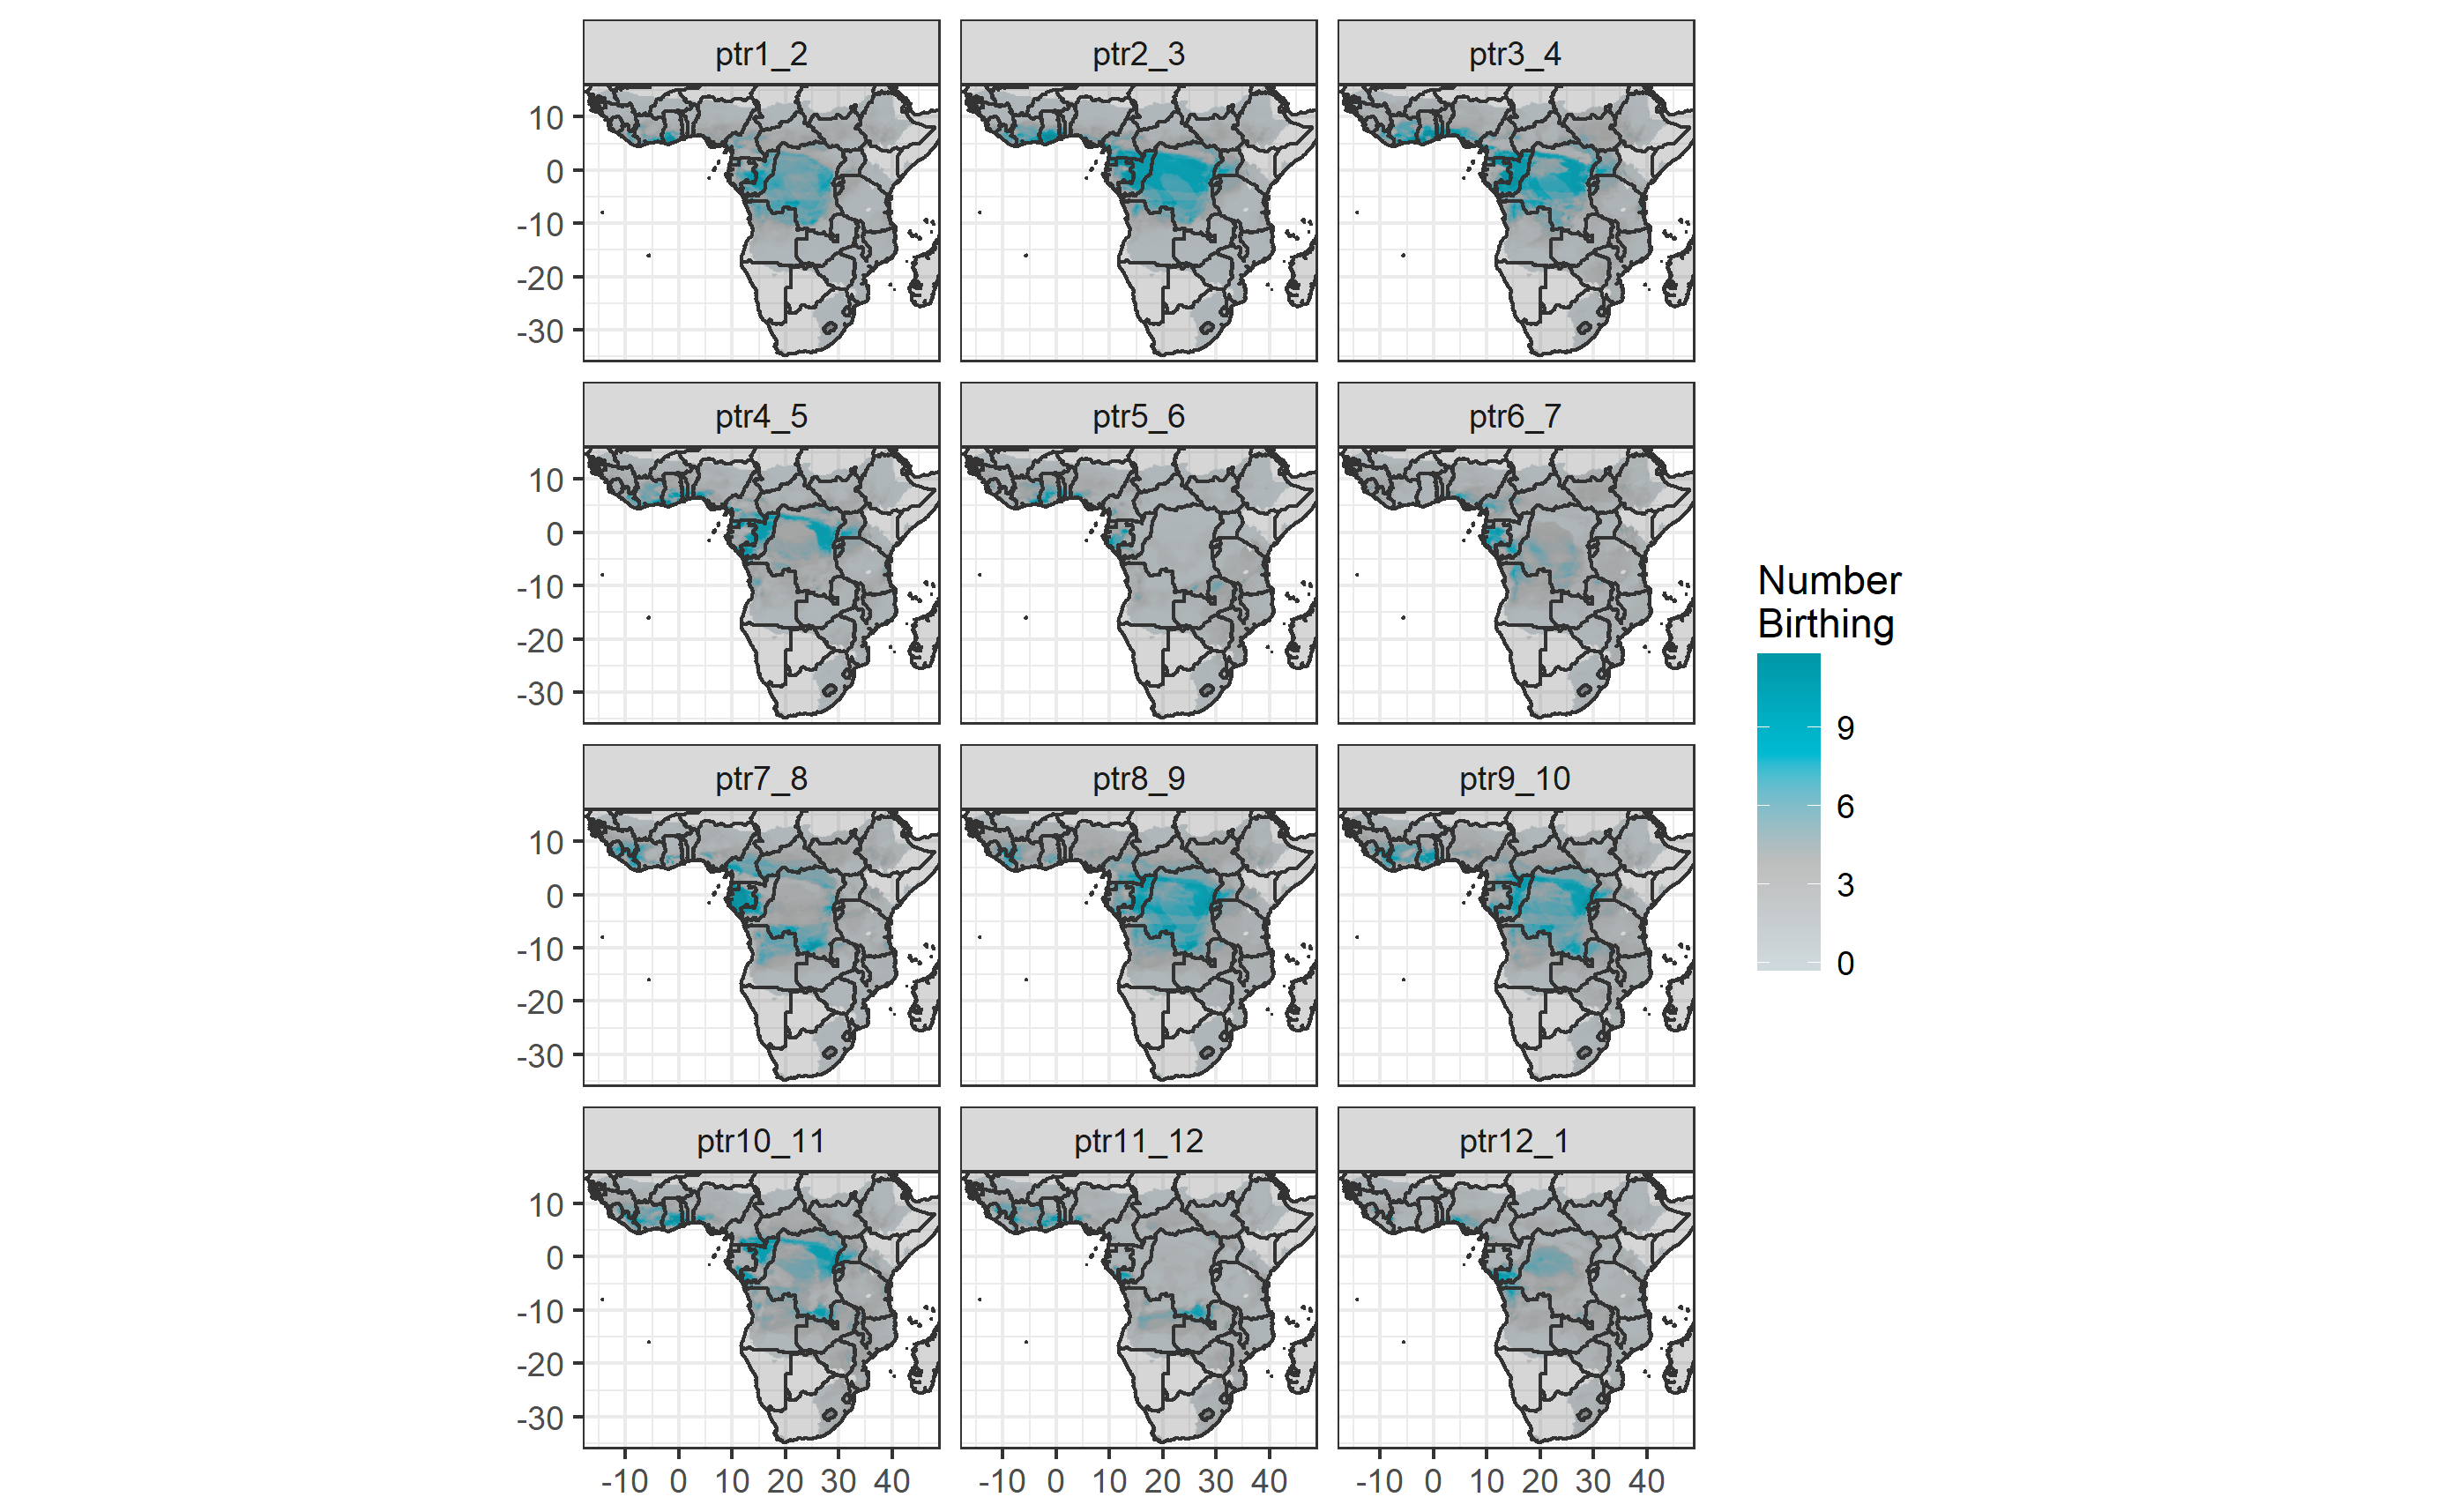
\includegraphics[width=.8\linewidth]{ptrBF_SI.png}
    \caption{Monthly force of birthing for African fruit bats}
    \label{fig:ptrBF}
\end{figure}
\FloatBarrier

\newpage\clearpage
\begin{figure}
    \centering
    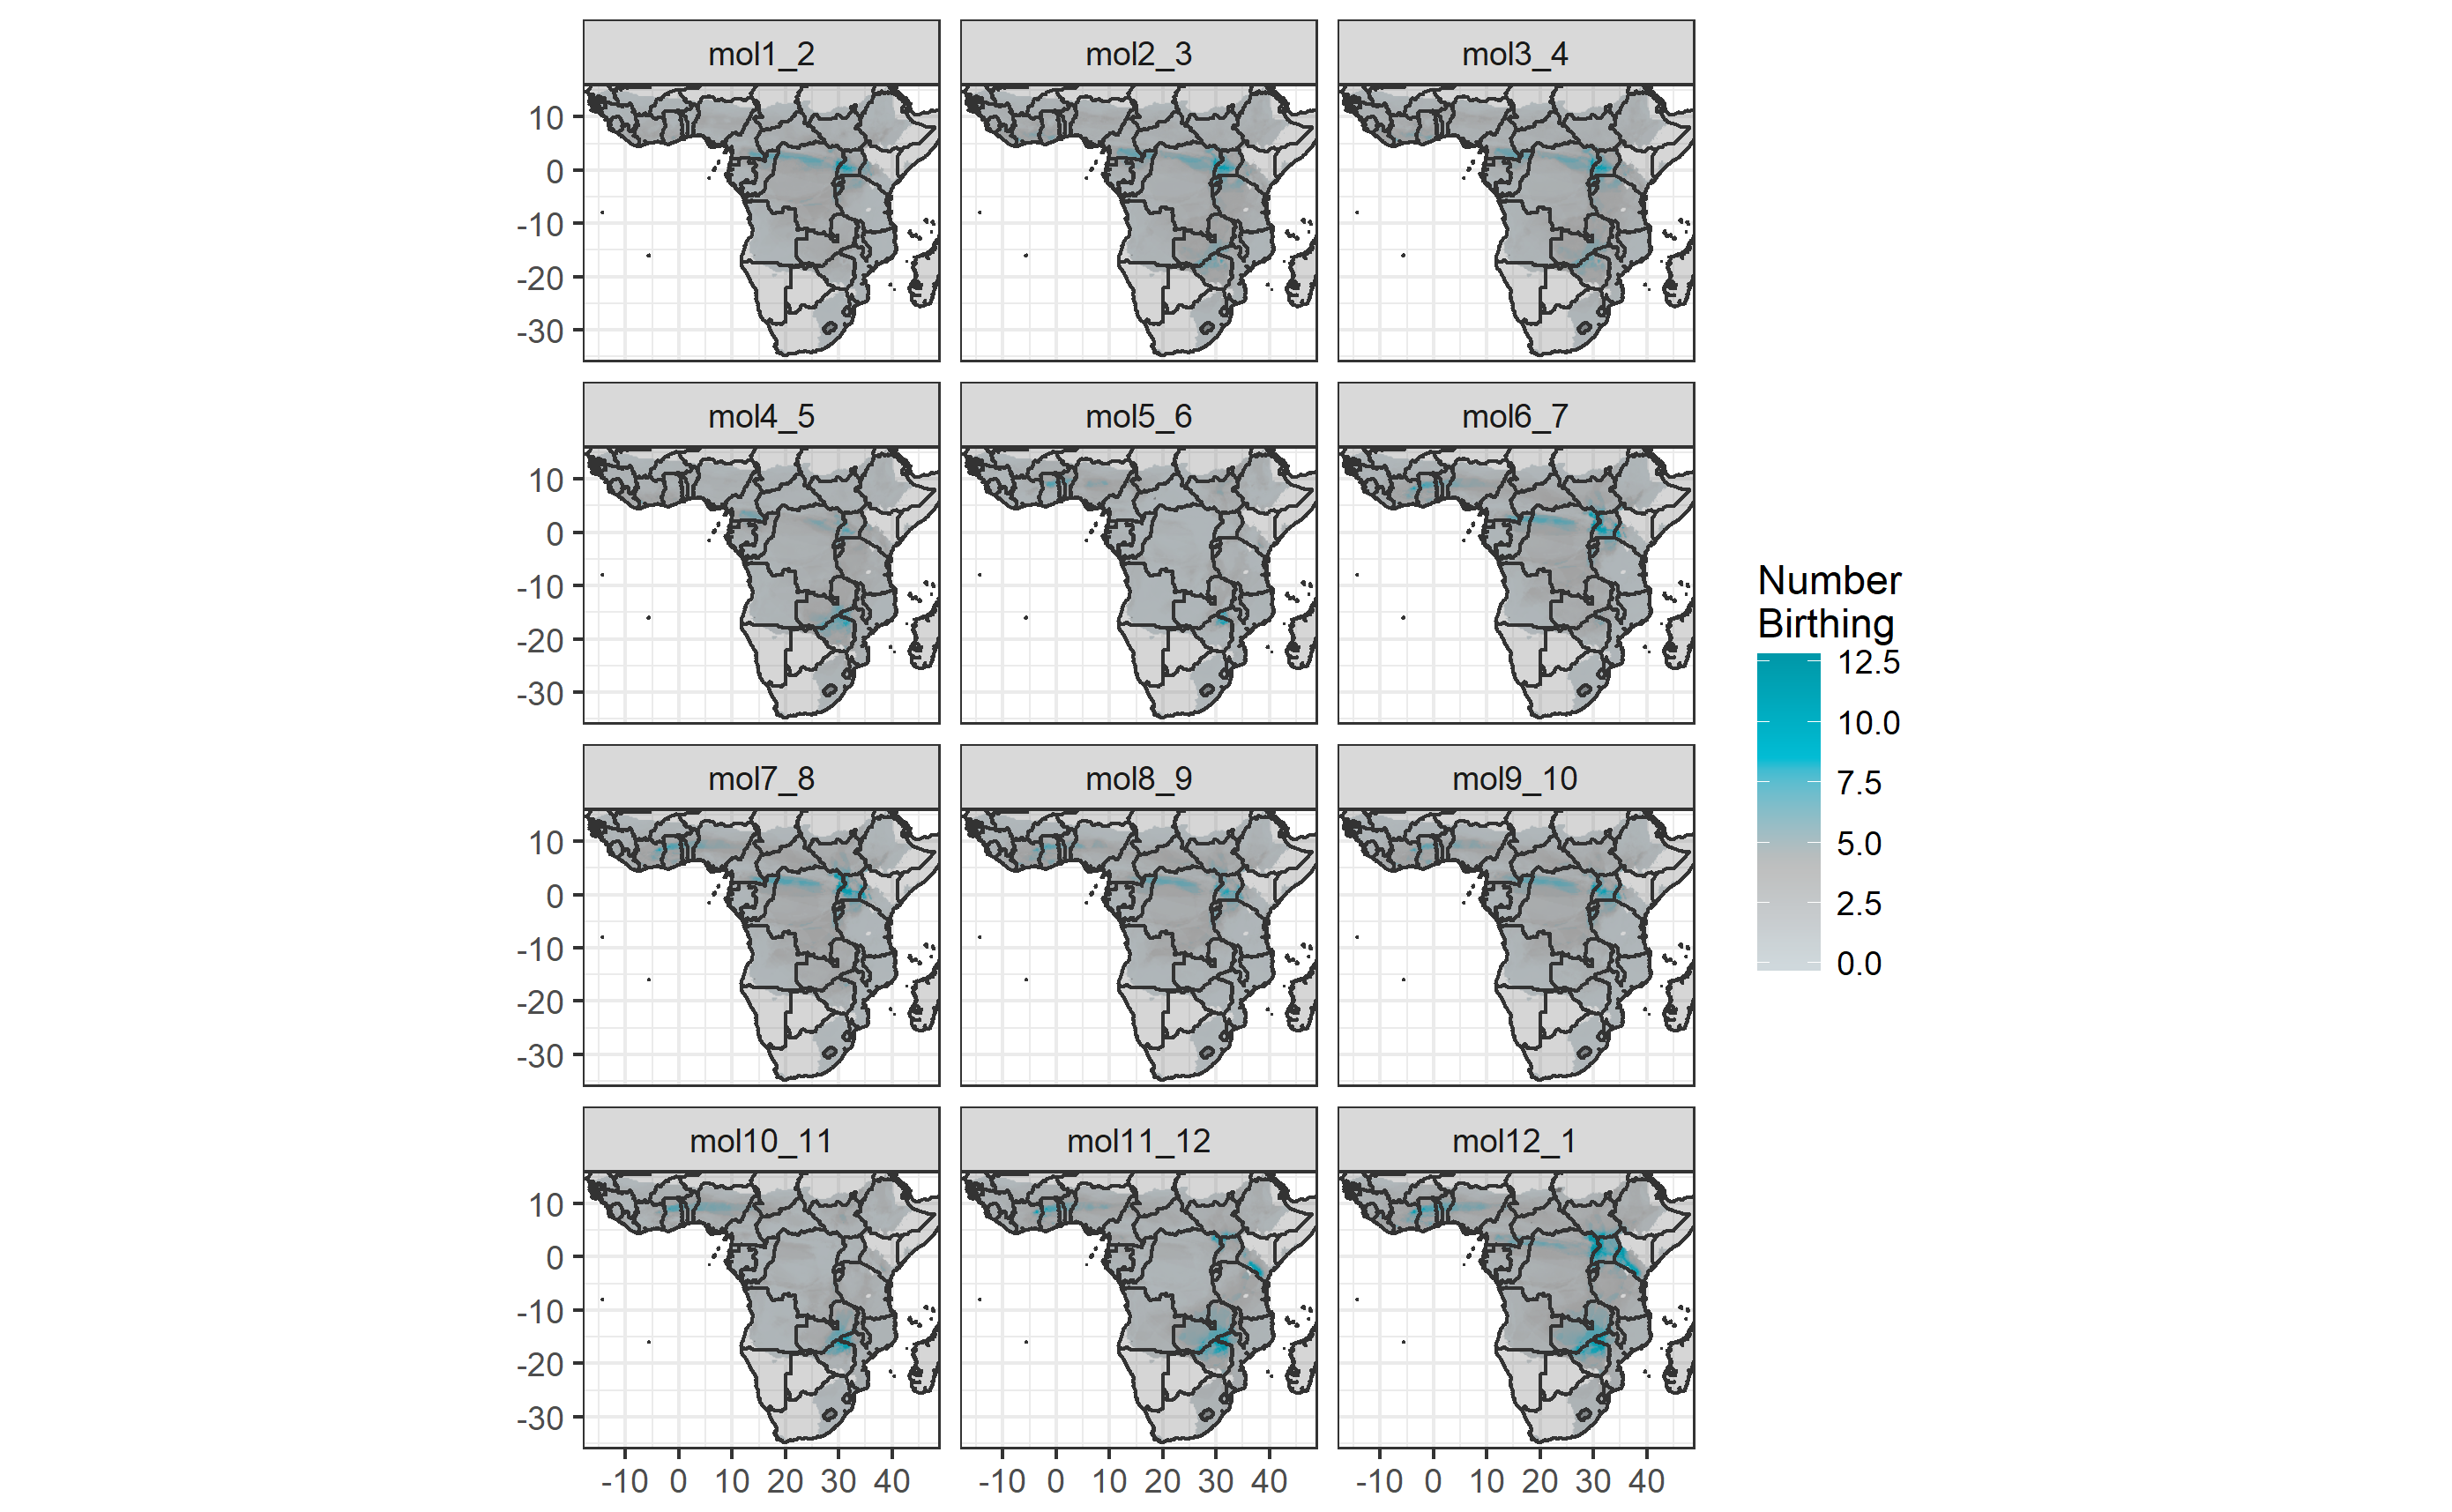
\includegraphics[width=.8\linewidth]{molBF_SI.png}
    \caption{Monthly force of birthing for mollosid bats}
    \label{fig:molBF}
\end{figure}
\FloatBarrier

\newpage\clearpage
\begin{figure}
    \centering
    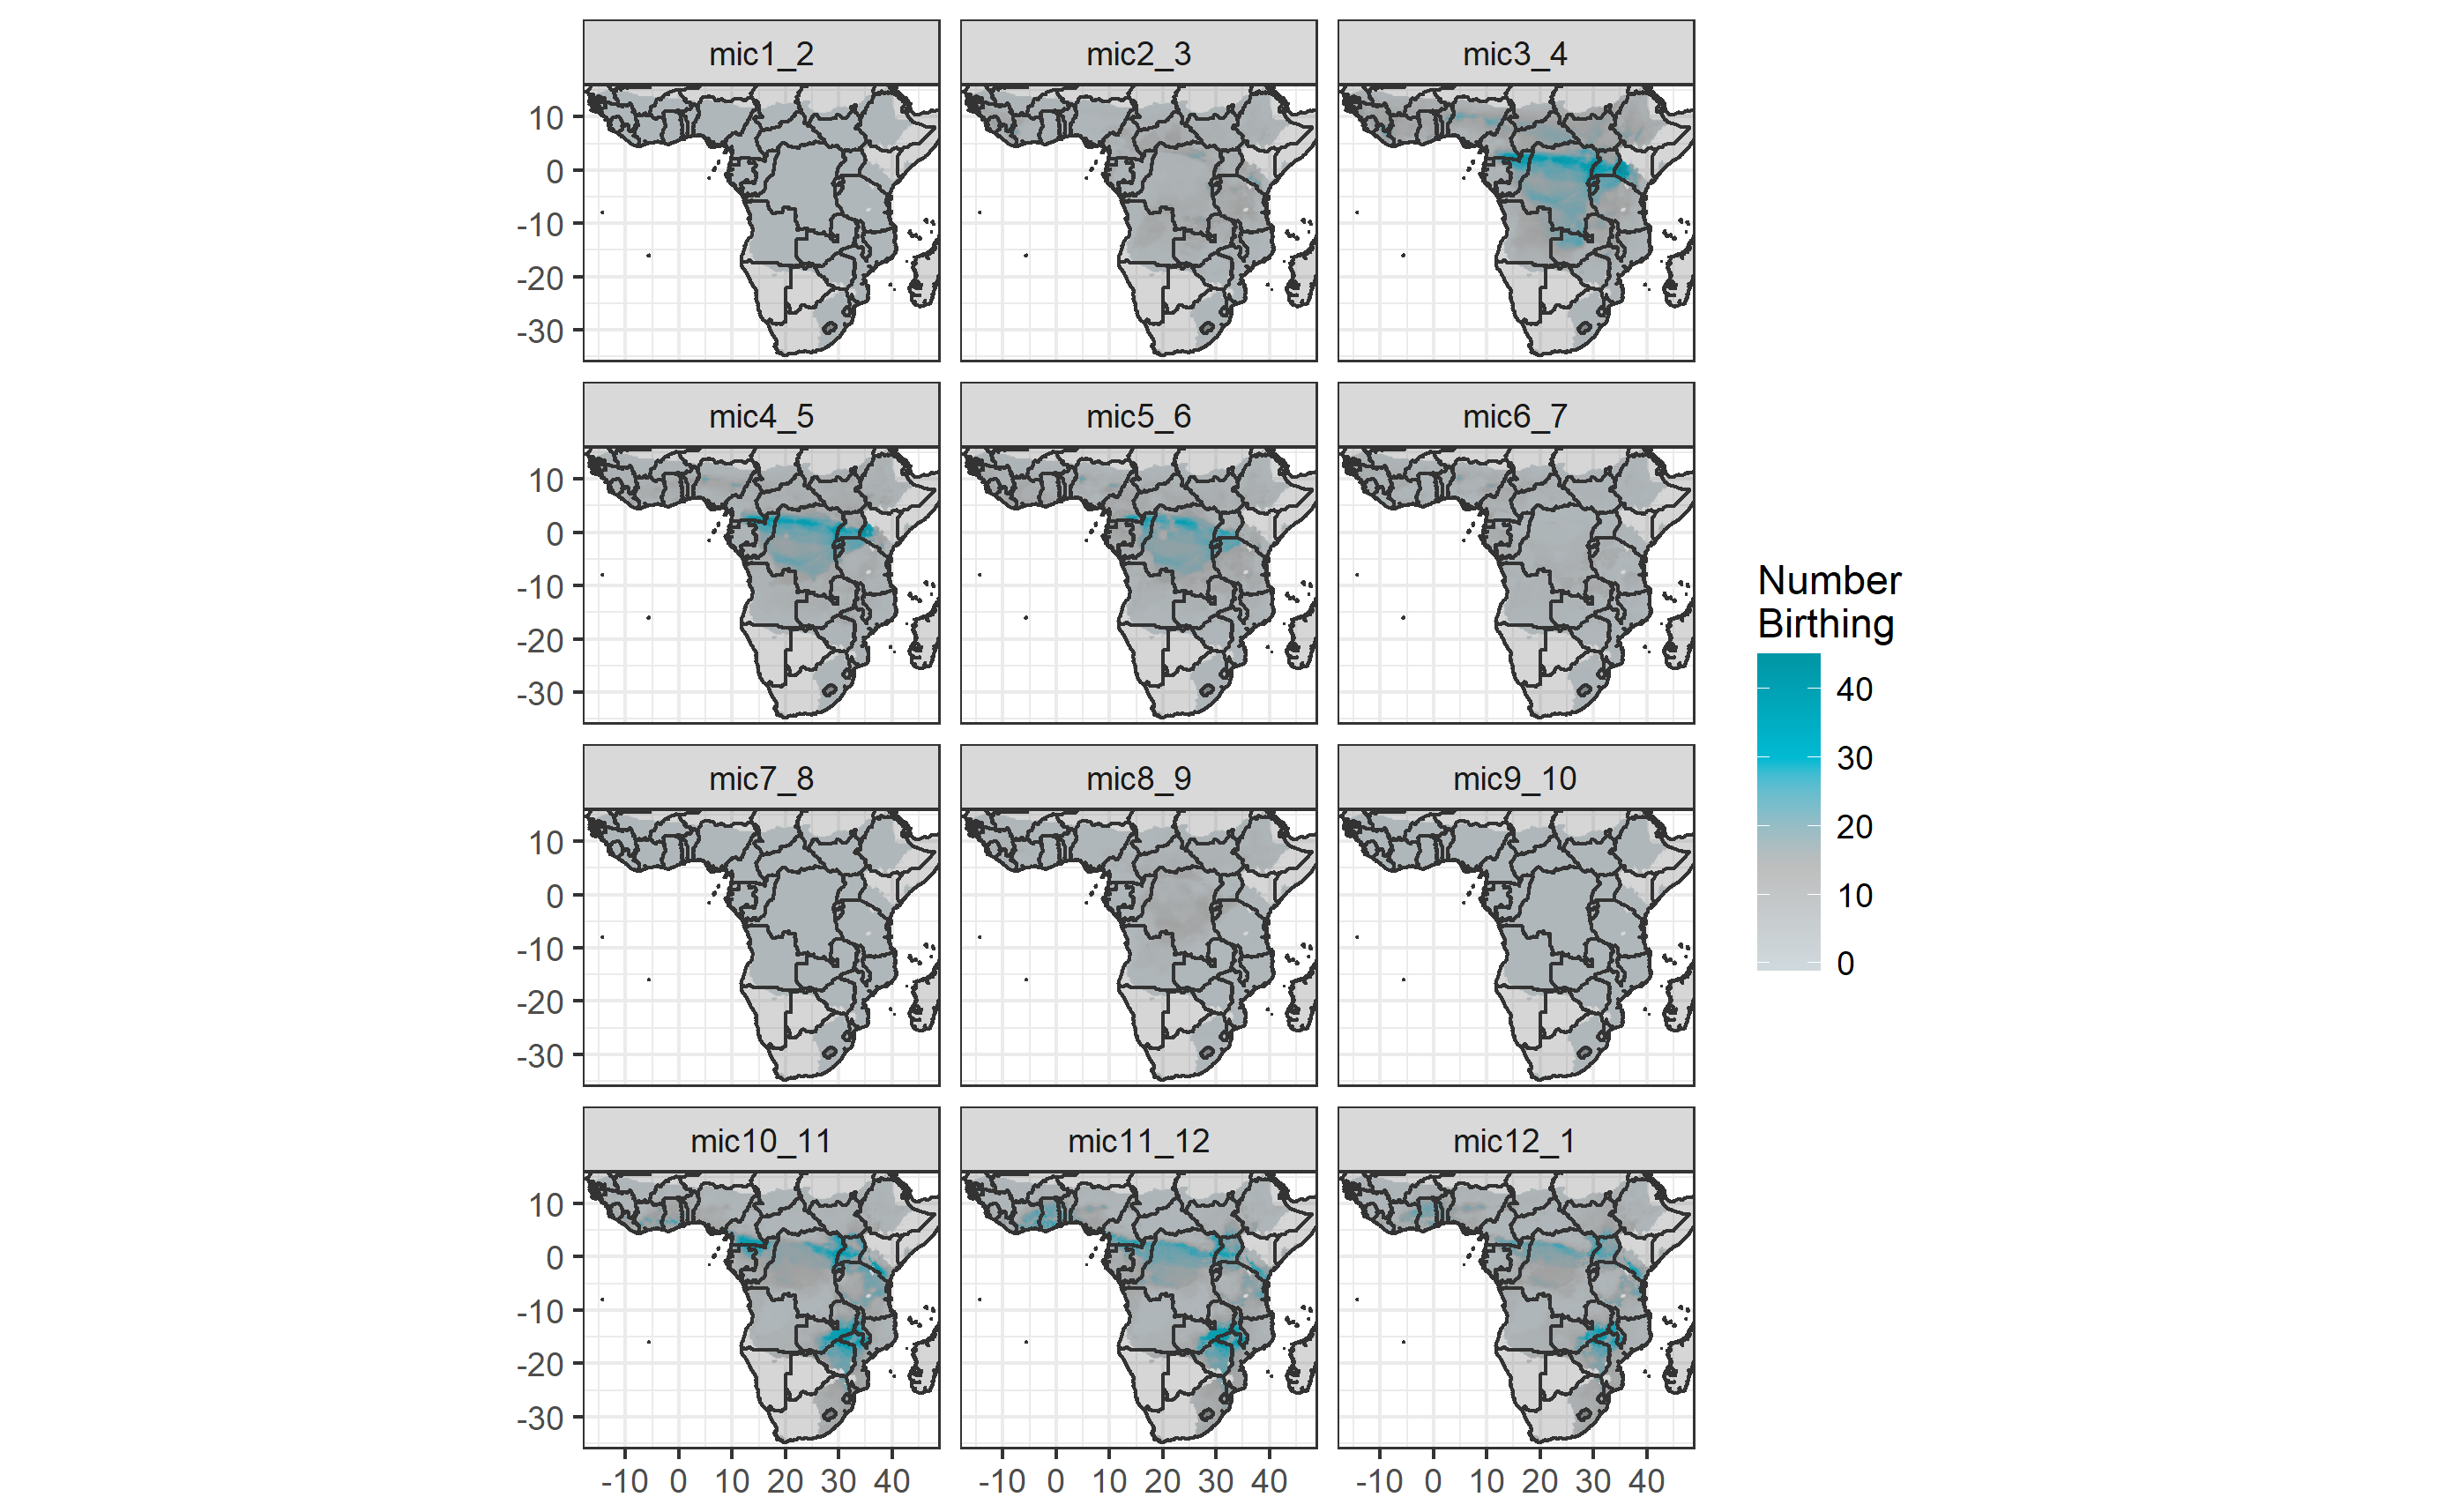
\includegraphics[width=.8\linewidth]{micBF_SI.png}
    \caption{Monthly force of birthing for non-mollosid microbats}
    \label{fig:micBF}
\end{figure}
\FloatBarrier

\newpage\clearpage
\begin{figure}
    \centering
    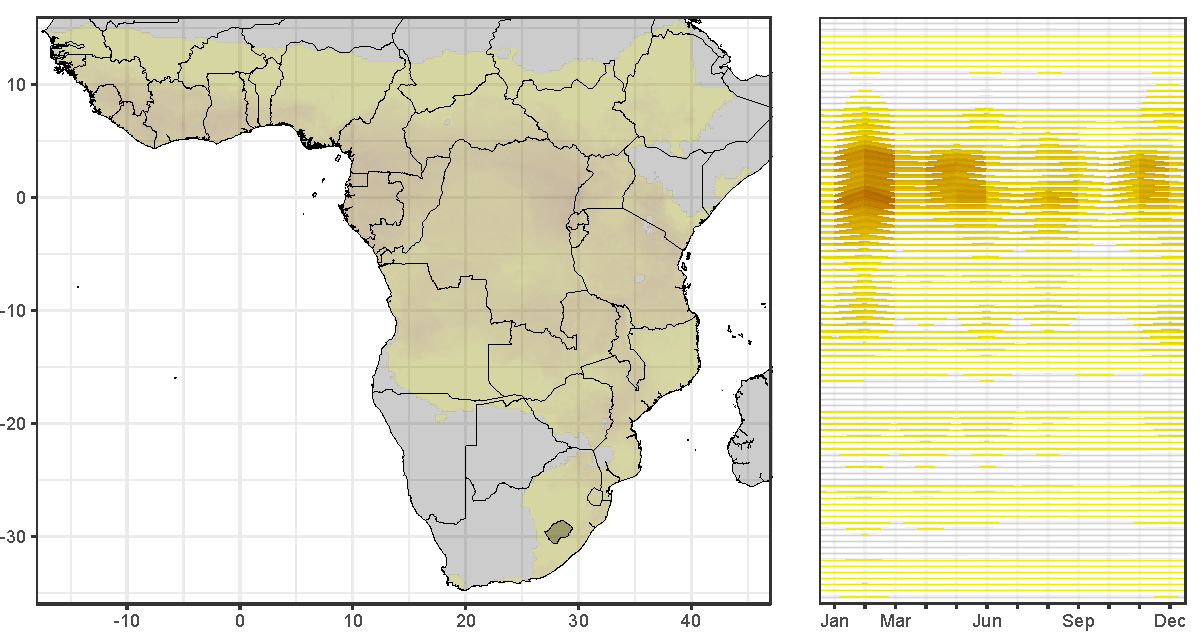
\includegraphics[width=.8\linewidth]{AnnRisk.pdf}
    \caption{Relative risk of ebolavirus spillover to non-human mammals}
    \label{fig:AnRisk}
\end{figure}

%%%

\begin{table}
\centering
\caption{Non-Human Spillover Full Model Results}
\label{table:spatGLM_AN}
\csvreader[tabular = l r r r  c,
	table head = Coefficients & Estimate & Std. Error & t Value &  P Value \\\hline\hline,
    late after line = \\,
    late after last line = \\\hline]%
    {AnFullResults.csv}{}%
    {\csvcoli &  \csvcolii &  \csvcoliii &  \csvcoliv &  \csvcolv}
\end{table}
\FloatBarrier

\begin{table}
\centering
\caption{Human Spillover Null  Model Results}
\label{table:spatGLM_Hum_Null}
\csvreader[tabular = l r r r  c,
	table head = Coefficients & Estimate & Std. Error & t Value &  P Value \\\hline\hline,
    late after line = \\,
    late after last line = \\\hline]%
    {HumNull.csv}{}%
    {\csvcoli &  \csvcolii &  \csvcoliii &  \csvcoliv &  \csvcolv}
\end{table}
\FloatBarrier

\begin{table}
\centering
\caption{Non-Human Spillover Null  Model Results}
\label{table:spatGLM_AN_Null}
\csvreader[tabular = l r r r  c,
	table head = Coefficients & Estimate & Std. Error & t Value &  P Value \\\hline\hline,
    late after line = \\,
    late after last line = \\\hline]%
    {AnNullResults.csv}{}%
    {\csvcoli &  \csvcolii &  \csvcoliii &  \csvcoliv &  \csvcolv}
\end{table}
\FloatBarrier
%%% Add this line AFTER all your figures and tables
\FloatBarrier


\dataset{dataset_one.txt}{Type or paste caption here.}

\dataset{dataset_two.txt}{Type or paste caption here. Adding longer text to show what happens, to decide on alignment and/or indentations for multi-line or paragraph captions.}

\bibliography{SI_FS_PNAS.bib}

\end{document}